%! TEX root = main.tex

\subsection{Validation: 2D Cylinder, $Re=\num{40}$}\label{sec:val_2d_cylinder_re40}

We used 2D cylinder flow at $Re=40$ to validate the solvers because it has a similar configuration with the $Re=200$ case that we will study later.
The $Re=40$ flow, however, does not exhibit vortex shedding and reaches a steady-state solution, making it suitable for validating the core functionality of the code.
Experimental data for this flow configuration is also widely available.

The spatial and temporal computational domains are $[-10$, $30]$ $\times$ $[-10$, $10]$ and $t \in [0, 20]$.
A cylinder with a nondimensional radius of $0.5$ sits at $x=y=0$.
Density is $\rho=1$, and kinematic viscosity is $\nu=0.025$.
The initial conditions are $u=1$ and $v=0$ everywhere in the spatial domain.
The boundary conditions are $u=1$ and $v=0$ on $x=-10$ and $y=\pm 10$.
At the outlet, i.e., $x=30$, the boundary conditions are set to 1D convective conditions:
\begin{equation}\label{eq:convec-bc}
    \pdiff{}{t}\begin{bmatrix} u \\ v \end{bmatrix}
    +
    c\pdiff{}{\vec{n}}\begin{bmatrix} u \\ v \end{bmatrix} = 0,
\end{equation}
where $\vec{n}$ is the normal vector of the boundary (pointing outward), and $c=1$ is the convection speed.

We ran the PetIBM validation case on a workstation with one (very old) NVIDIA K40 GPU and 6 CPU cores of the Intel i7-5930K processor.
The grid resolution is $562 \times 447$ with $\Delta t=\num{e-2}$.
The tolerance for all linear solvers in PetIBM was $\num{e-14}$.
We used the same linear solver configurations as those in the TGV verification case.

As for the PINN solvers, we validated two implementations with this cylinder flow because both codes were also used in the $Re=200$ case (as shown in section \ref{sec:case-study}).
The first implementation is an unsteady PINN solver, which is the same piece of code used in the verification case (section \ref{sec:verification}).
It solves the unsteady Navier-Stokes equations as shown in figure \ref{fig:pinn-workflow}.
The second one is a steady PINN solver, which solves the steady Navier-Stokes equations.
The workflow of the steady PINN solver works similar to that in figure \ref{fig:pinn-workflow} except that all time-related terms and losses are dropped.

Both PINN solvers used MLP networks with \num{6} hidden layers and \num{512} neurons each.
The Adam optimizer configuration is the same as that in section \ref{sec:verification}.
The learning rate scheduler is a cyclical learning rate with $\eta_{low}=\num{e-6}$, $\eta_{high}=\num{e-2}$, $N_c=\num{5000}$, and $\gamma={9.9998e-1}$.
We ran all PINN-related validations with one NVIDIA A100 GPU,
all using single-precision floats.

To evaluate PDE losses, \num{256000000} spatial-temporal points were randomly sampled from the computational domain and the desired simulation time range.
In each iteration, \num{25600} points were used to evaluate the PDE losses, so the Adam optimizer would see each points \num{40} times on average during the \num{400000}-iteration optimization.
\num{25600000} points were sampled on the boundaries at $y=\pm 10$, and \num{12800000} were sampled on the boundaries of $x=-10$ and $x=30$.
On the cylinder surface, the number of spatial-temporal points were \num{5120000}.
In each iteration, \num{2560}, \num{1280}, and \num{512} points were used, respectively.

Figure \ref{fig:cylinder-re40-pinn-loss} shows the training history of the PINN solvers.
The total loss of the steady PINN solver converged to around \num{e-4}, while that of the unsteady PINN solver converged to around \num{e-2} after about 26 hours of training.
Readers should be aware that the configuration of the PINN solvers might not be optimal, so the accuracy and the computational cost shown in this figure should not be treated as an indication of PINNs' general performance.
In our experience, it is possible to reduce the run time in half but obtain the same level of accuracy by adjusting the number of spatial-temporal points used per iteration.

\begin{figure}
    \centering%
    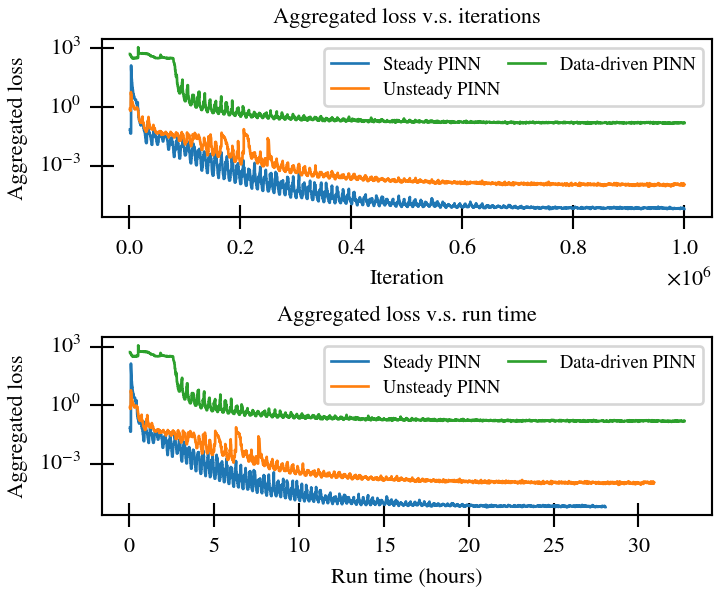
\includegraphics[width=\columnwidth]{cylinder-2d-re40/loss-hist.png}%
    \caption{%
        Training convergence history of 2D cylinder flow at $Re=\num{40}$ for both steady and unsteady PINN solvers.
    }
    \label{fig:cylinder-re40-pinn-loss}%
\end{figure}

Figure \ref{fig:cylinder-re40-contours} shows the comparison of the steady-state flow fields (i.e., the snapshots at $t=20$ for PetIBM and the unsteady PINN solver).
The PINN solvers' results visually agree with PetIBM's.
The variation in the vorticity of PINNs only happens at the contour line of \num{0}, so it is likely caused by trivial rounding errors.
Note that vorticity is obtained by post-processing for all solvers.
PetIBM used central difference to calculate the vorticity, while the PINN solvers used automatic differentiation to obtain it.

Figure \ref{fig:cylinder-re40-drag-lift} gives the drag and lift coefficients ($C_D$ and $C_L$) with respect to simulation time.
Note the steady PINN solver's results were omitted as it does not have time history.
The PINN's results visually agrees with PetIBM's.
Table \ref{table:cylinder-re40-cd-comparison} compares the values of $C_D$ against the experimental data and simulation data from the literature.
As seen from the table, values from different works in the literature do not closely agree with each other.
Though there is not a single value to compare against, at least the $C_D$ from the PINN solvers and PetIBM fall into the range of other published works.
We consider the results of $C_D$ validated for the PINN solvers and PetIBM.

\begin{figure}
    \centering%
    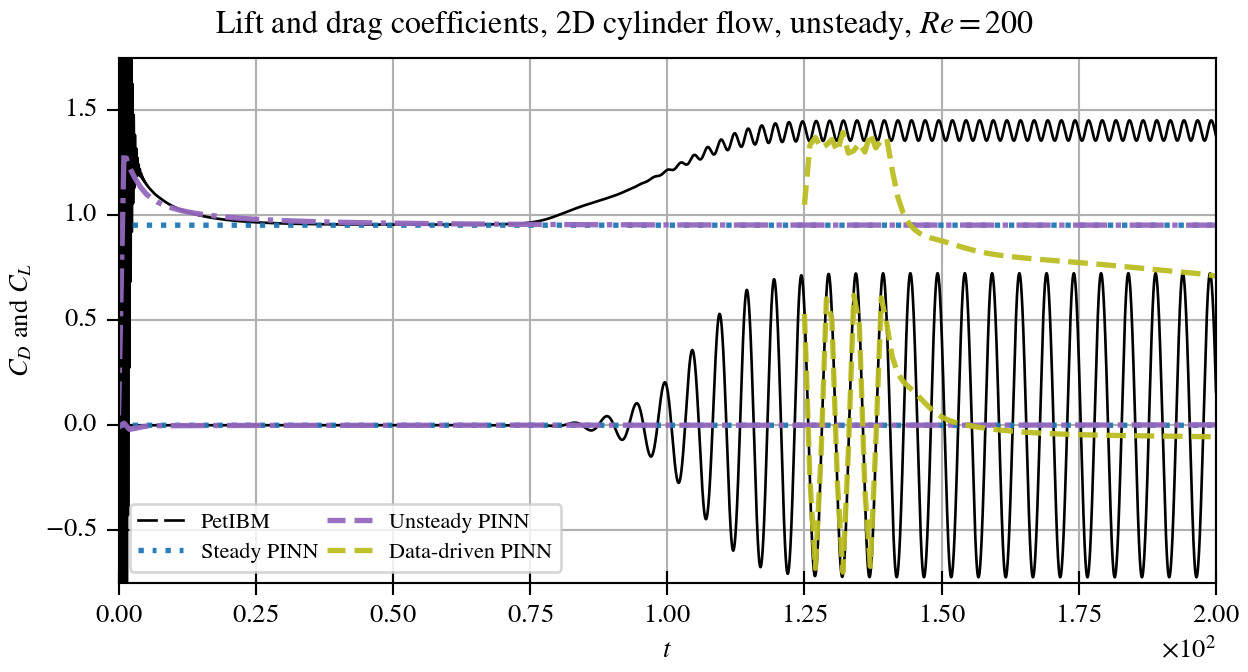
\includegraphics[width=\columnwidth]{cylinder-2d-re40/drag-lift-coeffs}%
    \caption{%
        Drag and lift coefficients of 2D cylinder flow at $Re=\num{40}$ w/ PINNs.
    }
    \label{fig:cylinder-re40-drag-lift}%
\end{figure}

\begin{table}
    \centering%
    \begin{threeparttable}[b]
        \begin{tabular}{lccc}
            \toprule
            & $C_D$ & $C_{D_p}$ & $C_{D_f}$ \\
            \midrule
            Steady PINN & 1.62 & 1.06 & 0.55 \\
            Unsteady PINN & 1.60 & 1.06 & 0.55 \\
            PetIBM & 1.63 & 1.02 & 0.61 \\
            Rosetti et al., 2012\cite{rosetti_urans_2012}\tnote{1} & \num{1.74+-0.09} & n/a & n/a \\
            Rosetti et al., 2012\cite{rosetti_urans_2012}\tnote{2} & 1.61 & n/a & n/a \\
            Sen et al., 2009\cite{sen_steady_2009}\tnote{2} & 1.51 & n/a & n/a \\
            Park et al., 1988\cite{park_numerical_1998}\tnote{2} & 1.51 & 0.99 & 0.53 \\
            Tritton, 1959\cite{tritton_experiments_1959}\tnote{1} & 1.48--1.65 & n/a & n/a \\
            Grove et al., 1964\cite{grove_experimental_1964}\tnote{1} & n/a & 0.94 & n/a \\
            \bottomrule
        \end{tabular}%
        \begin{tablenotes}
            \footnotesize
            \item [1] Experimental result
            \item [2] Simulation result
        \end{tablenotes}
        \caption{%
            Validation of drag coefficients. %
            $C_D$, $C_{D_p}$, and $C_{D_f}$ denote the coefficients of total drag, pressure drag, %
            and friction drag, respectively.%
        }%
        \label{table:cylinder-re40-cd-comparison}
    \end{threeparttable}
\end{table}%

Finally, figure \ref{fig:cylinder-re40-pinn-surfp} shows the pressure distribution on the cylinder surface.
Again, though there is not a single solution that all works agree upon, the results from PetIBM and the PINN solvers visually agree with the published literature.
We consider PetIBM and both PINN solvers validated.

\begin{figure}
    \centering%
    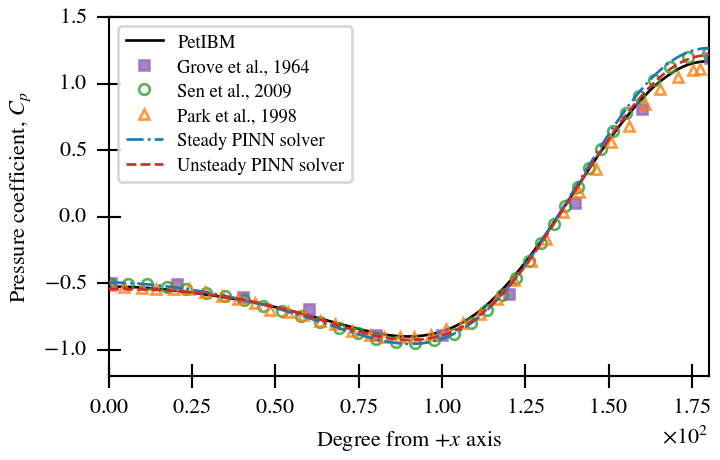
\includegraphics[width=0.95\columnwidth]{cylinder-2d-re40/surface-pressure}%
    \caption{%
        Surface pressure distribution of 2D cylinder flow at $Re=\num{40}$
    }
    \label{fig:cylinder-re40-pinn-surfp}%
\end{figure}

\begin{figure*}
    \centering%
    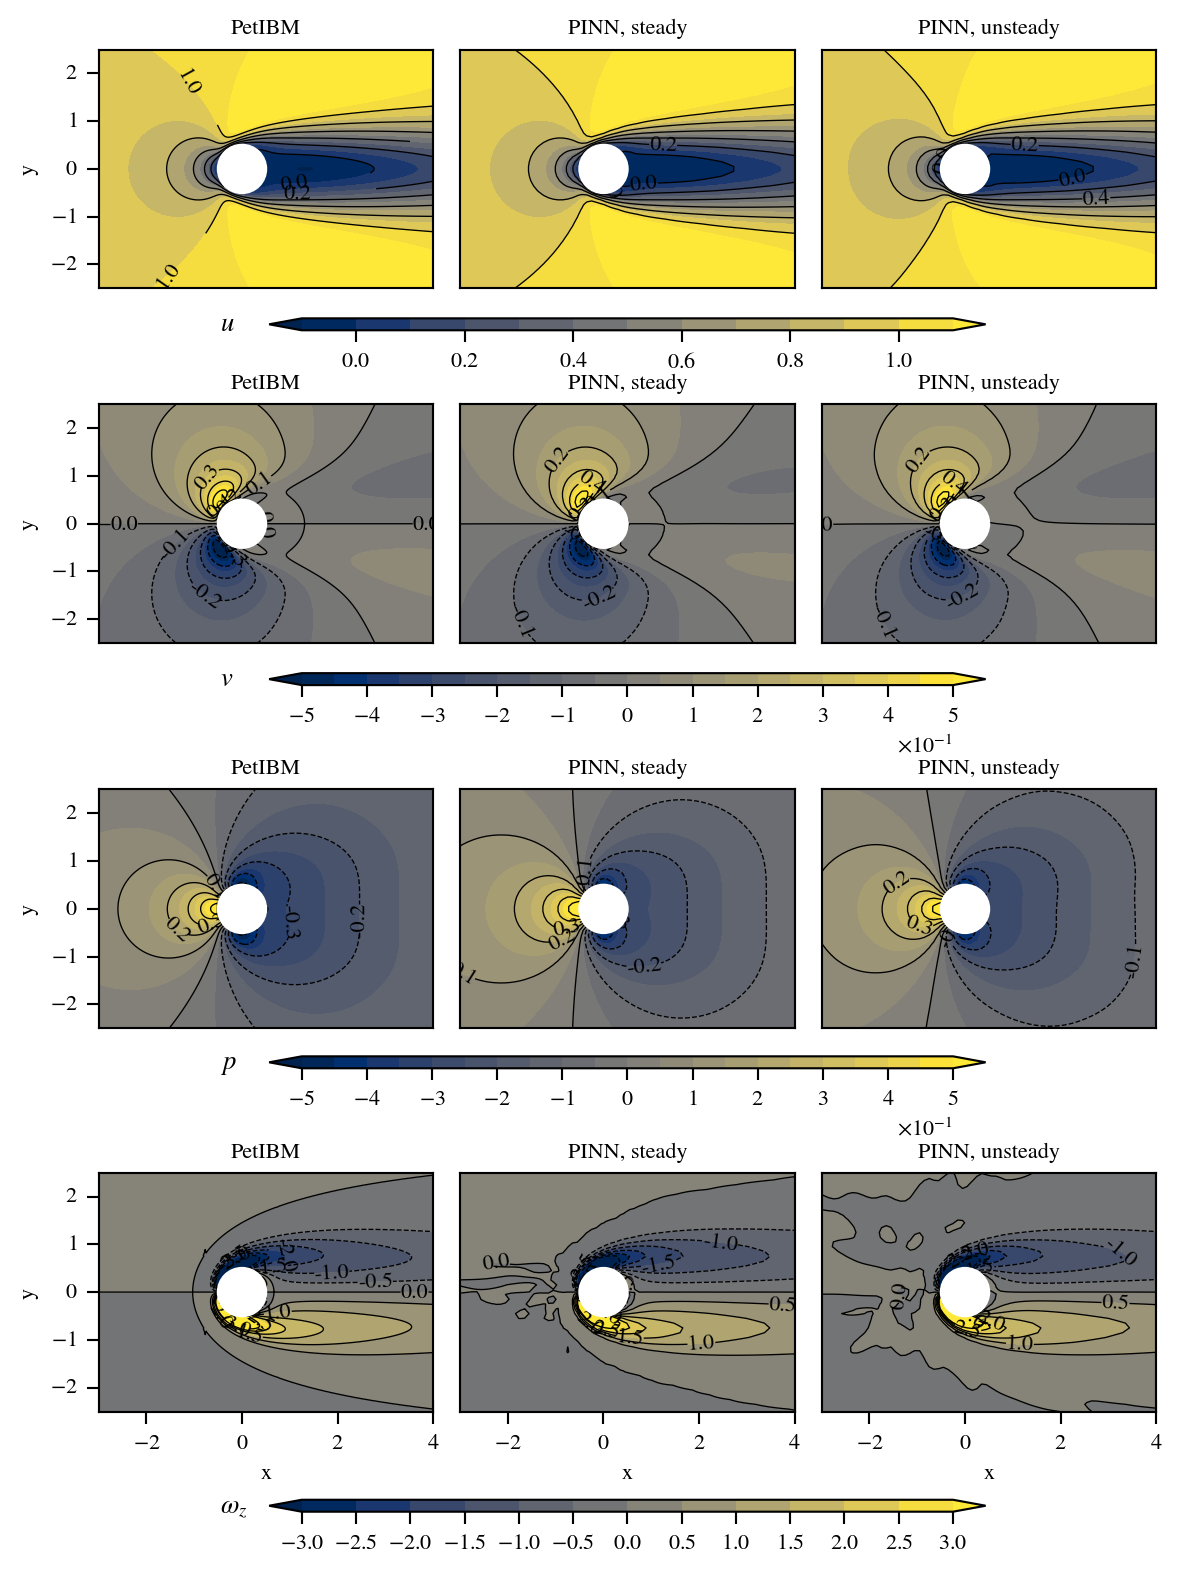
\includegraphics{cylinder-2d-re40/contour-comparison}%
    \caption{%
        Contour comparison of 2D cylinder flow at $Re=\num{40}$
    }
    \label{fig:cylinder-re40-contours}%
\end{figure*}

% vim:ft=tex:
